\section{The Beautiful Soul}

In order to satisfy a social obligation, I saw the movie \textit{RIPD}\footnote{\url{https://www.imdb.com/title/tt0790736/?ref_=nv_sr_srsg_0}} last week (no, I don't recommend it). Although it has no deeper meaning, we can possibly insert one for it. Although I doubt and such meaning was consciously assumed by the creators, it is possible that higher powers subtly influenced them. The premise of the film is that there are walking dead among us, men without souls, or actually souls so ugly they would be better off without them. Hence, it is no great gift to be able to see men's souls.

In the film, the dead souls create an artifact whose purpose is to call the ugly souls back to the earth. It is powered by the blood of, if not exactly a virgin, at least an innocent woman. Eerily, these are two themes that we have mentioned. The first is the idea that there are hungry ghosts\footnote{\url{https://gornahoor.net/?p=2507}} about, since they are no longer revered by their ancestors. The second is the idea of the problem of births\footnote{\url{https://gornahoor.net/?p=1664}}, and how spirits are attracted to specific material and psychic conditions following the law of affinity.

The Medieval period attracted souls destined to salvation and so attracted nobles, saints, knights, contemplatives, hermetists, etc. However, it also attracted the rebels, those opposed to all order and authority. That is the spiritual battle that was eventually lost. The rebels, beginning with Luther, through the French and Soviet revolutions made possible the births of new types of souls. This will sound incredible to the modern mind because it seems unscientific on the surface and goes against all notions of egalitarianism. He prefers to see this trend as the ``evolution" of man. In a sense he is correct, but in a sense opposite to what he intended. It has to do with the ``survival of the fittest", and only certain types of souls are fit for the current ugly environment. This is what Guenon means by ``compossible".

Nevertheless, the modern world also attracts a band of counterrevolutionary warriors ready to do spiritual battle. Unfortunately, they come ill prepared. They lack the resources for spiritual development and often grasp at any ideas that sound plausible. They are disorganized and hence fall prey to the various counter Traditional movements that claim to be on the right. These are the ones who must be awakened to their destiny. Whatever the modern world hates, they should probably love; whatever the modern world despises and condemns, is probably where the truth lies hidden.

So that they don't flounder like the mass of men today, the secret counterrevolutionaries need to develop their sense of ``I" and their will. This is the alchemical task of the creation of the homunculus which is generated through the alchemical marriage. Now there is a lot of ineffective erudition surrounding alchemy, because it can never be understood without doing the ``lab work". Of course, lab work is not the same as that done by the ``puffers", but really through the efforts of the alchemical transformation of one's own consciousness.

\begin{wrapfigure}{rt}{.3\textwidth}
 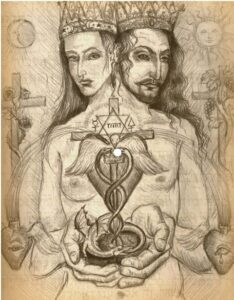
\includegraphics[scale=.5]{a20130723TheBeautifulSoul-img001.jpg}
\end{wrapfigure}

This is the marriage of the spirit, which is masculine, and the soul (``anima"), which is feminine. We have mentioned the fruits of this task many times in conjunction with Tomberg's Meditations on the Holy Spirit, the Virgin, and the birth of the Christ. That is the religious teaching on the macro level, but on the micro level, i.e., the esoteric teaching, it has a different significance. It is about the birth of one's true self, putting on the mind of Christ. Yet, there is that old joke about where can you find a virgin today? Hence, that is the first alchemical task, the beginning of the ``lab work", which involves the purification of the soul, i.e., a virginal soul.

Anyone who has been reading attentively will have an idea of what that entails. This does not mean that the task is easy and without risks. What is understood in the abstract does not necessarily transfer to self-understanding. The ego, the false self, has been carefully constructed over a lifetime and serves as a sort of buffer zone to protect the psyche from the lower psychic elements in the environment. Unfortunately, it also protects the self from hearing anything higher.

Without the feedback and support of a group, there are dangers in this. First of all, as the egoic psyche is broken up, there is a real danger of insanity unless something higher and more solid can replace it. Another danger is that the ego, while resisting its dissolution, will still claim ownership of higher states; this is a form of ego inflation. There is no point to continue in this vein. Nevertheless, the prize is worth the game for those who persist. Once devoid of subjectivity, negative emotions, irrational fears, unsupportable opinions, and so on, a man is able to operate freely in the world, secure in himself. What a group of such men can accomplish is not yet known.

I have never asked a woman for money. I have often asked for her soul, which she willingly gives, probably because she believes it doesn't cost anything. She doesn't realize that she is the man's soul; a man mistakenly assumes he wants the body, when it is really completeness that is his true desire.

A man is complete in himself, at least virtually. He has both an X and a Y chromosome, so he can create both the male and the female. As below, so above, so he also comprises both possibilities spiritually. The woman, with two X chromosomes, can only beget another woman. Only a miracle, the action of the spirit on her can beget a male child, the I, the true Self.

For this to occur, the woman must be compliant or must be made compliant. Such a woman is beautiful, and the man who has possessed her, has a beautiful soul. St Theresa d'Avila claimed that if you could see your soul in its purity, you would think you saw God.

The meeting of the spirit and the soul is the sign of the cross, the soul moving horizontally and the Spirit descending vertically until they meet and join together. Yet that initial meeting is incomplete, as they still must take part in the alchemical marriage, the mysterium coniunctionis.



\flrightit{Posted on 2013-07-23 by Cologero }

\begin{center}* * *\end{center}

\begin{footnotesize}\begin{sffamily}



\texttt{JA on 2013-07-24 at 19:27 said: }

Cologero, how would you differentiate on the esoteric level between the alchemical marriage and the ``pandrogony" of a Genesis P-Orridge ? or some aspects of transgender (people that claim to be both male and female)….also what do you make of this Gurdjieff-derived teaching that apparently claims the Maitreya Buddha will be some sort of transsexual ? 

\url{http://www.eboards4all.com/717093/messages/49634.html}


\hfill

\texttt{Cologero on 2013-07-24 at 22:44 said: }

Since you want to bring Gurdjieff into it, he wrote that this obsession with sex is the cause of mechanicalness and self-deception:

\begin{quotex}
At the same time sex plays a tremendous role in maintaining the mechanicalness of life. Everything that people do is connected with `sex'. politics, religion, art, the theater, music, is all `sex.' Do you think people go to the theater or to church to pray or to see some new play? That is only for the sake of appearances. The principal thing, in the theater as well as in church, is that there will be a lot of women or a lot of men. This is the center of gravity of all gatherings. What do you think brings people to cafés, to restaurants, to various fetes? One thing only. Sex: it is the principal motive force of all mechanicalness. All sleep, all hypnosis, depends upon it. 

\end{quotex}
Ultimately, what counts is not talking about it, but rather actually achieving something. If you want to believe that Genesis P-Orridge is some enlightened being, then you can follow his path and send us a postcard every now and then describing your progress.

The alchemical marriage is about the transmutation of inner states, not corporeality. Maybe not what you want to hear, but if you get your inner life organized, the outer will follow.


\hfill

\texttt{JA on 2013-07-25 at 00:49 said: }

Cologero I hope you have not the wrong impression of me ! As a man and as a warrior if you are insinuating what I suppose you may be insinuating if we knew each other in person I might have to challenge to a duel to defend my honour !

Back to the matter at hand, you've made a definitive answer in that true enlightenment is in the interior. Too many ``occultists" (P-Orridge whom I mentioned but many many others as well) focus on the body. Decadence disguised as Tantra as you've mentioned before. I'm interested to hear your upcoming commentaries on the Serrano book which I have read before. 

I am on the right track as I don't particularly think about sex all that much in my life, if I talk about it's because I am bewildered by the heroin-like cravings I see in those around me……


\hfill

\texttt{CaseyAnn on 2013-10-22 at 20:00 said: }

Hi Cologero,

I think there's a typo here:

``Now there is a lot of ineffective erudition surrounding alchemy, because it can never be understood with doing the `lab work.'"

I assume you meant ``it can never be understood without doing the `lab work.'" (At least, that's the only way it makes sense to me in the surrounding context.)

Blessings

—–

Thanks for picking up on that. It is now fixed. — Cologero


\end{sffamily}\end{footnotesize}
